\chapter{Metodologia}

Assim como foi discutido no capítulo anterior, para obter os parâmetros de caracterização da acústica interna de dutos circulares com escoamento, é preciso de um modelo que suporte a interação fluxo de massa e variação de pressão. Portanto modelos baseados em métodos de fluido dinâmica computacional se mostram adequados, principalmente aqueles baseados no método de \textit{lattice} Boltzmann assim como foi mostrado anteriormente nos trabalhos de \citeonline{da2006lattice} e \citeonline{da2009sound}. Nesse sentido, há traballhos que validam, aplicam e desenvolvem metodologias de \textit{lattice} Boltzmann no campo de estudo da aeroacústica.

Um desses estudos é o de \citeonline{crouse2006fundamental}, que mostraram a eficácia do método de \textit{lattice} Boltzmann em recuperar as equações de Navier-Stokes de transiente, compressível e viscosa. Há de se ressaltar que validaram também o modelo numérico de um ressonador de Helmholtz com um modelo experimental do mesmo, demonstrando assim a viabilidade da aplicação para problemas de acústica.

No que se trata de desenvolvimento de ferramentas auxiliares para tratar problemas acústicos, \citeonline{kam2006non} desenvolveu uma condição de contorno que caracteriza dissipação de energia acústica e fluido dinâmica, ou seja, uma condição de contorno anecóica. Ela se baseia no acoplamento de mais um termo na equação de Boltzmann para gerar uma região de amortecimento, redirecionando os valores de densidade e velocidade das partículas para um valor alvo, que seria no caso valores médios de densidade e velocidade num fluido em repouso.

\citeonline{marie2009} analisou e comparou esquemas de alta ordem das equações de Navier-Stokes linearizadas com o método de \textit{lattice} Boltzmann. O objeto de estudo para comparação foi análises de dispersão e dissipação de ondas acústicas em regime isotérmico. Conclui-se com esse trabalho que para um determinado erro de dispersão o método de \textit{lattice} Boltzmann se comportou como mais rápido.

No que diz respeito a aplicação do método de \textit{lattice} Boltzmann num problema de aeroacústica, \citeonline{lew2010noise} desenvolveram um modelo numérico em 3D para predição de ruído em um jato turbulento subsônico. Como validação os resultados foram comparados com resultados experimentais e cálculos numéricos feitos a base de \textit{Large} \textit{Eddy} \textit{Simulation} (LES)\abreviatura{LES}{\textit{Large} \textit{Eddy} \textit{Simulation}}. Esse estudo demonstrou as principais vantagens de se trabalhar com o método de \textit{lattice} Boltzmann como por exemplo o baixo custo computacional e a facilidade em inserir \textit{nozzles} com formas complexas no domínio computacional.

Também na área de aeroacústica computacional, o trabalho de \citeonline{shi2013lattice} propõe um modelo em \textit{lattice} Boltzmann para obter dados de diretividade da radiação sonora num duto circular submetido a escoamento subsônico. Os resultados de diretividade foram comparados com os modelos de \citeonline{levine1948radiation} e \citeonline{gabard2006}, mostrando uma boa convergência principalmente nas baixas frequências.

Já no sentido de tratamento de fenômenos da acústica básica, \citeonline{viggen2013acoustic} investigou os efeitos da adição de termos fontes no método de \textit{lattice} Boltzmann, mapeando eles nos parâmetros macroscópicos através da ferramenta matemática de expansão de Chapman-Enskog. Como resultado conseguiu reproduzir fenômenos de diretivade de monopolos, dipolos e quadrupolos.

\citeonline{da2015assessment} abordaram também o uso do método de \textit{lattice} Boltzmann acoplado com \textit{Large} \textit{Eddy} \textit{Simulation} (LES) na investigação do ruído gerado na interação do escoamento de um jato com uma placa plana. Os dados de níveis de pressão sonora em campo distante foram obtidos usando a superfície de Ffowcs-Williams e Hawkings (FW-H)\abreviatura{FW-H}{Superfície de Ffowcs-Williams e Hawkings} e os mesmos possuem uma boa convergência com dados experimentais.

Investigar a acústica interna de dutos circulares com escoamentos é um processo que deve ter suporte de ferramentas bem específicas, como por exemplo o método numérico de \textit{lattice} Boltzmann. Esse capítulo portanto abordará esse método e as condições de uso implementadas, validadas e verificadas num \textit{software} de código aberto chamado \citeonline{palabos}. Abordar o uso de um \textit{software} de código aberto possibilita a verificação transparente dos processos de cálculo bem como adaptações com novas implementações dentro do projeto, focando a melhor aderência da ferramenta computacional para resolução do problema.


\section{O Método de Lattice Boltzmann}

O método de \textit{lattice} Boltzmann possui bastante utilidade quando se trata de problemas aeroacústicos, pequenas flutuações de pressão e fenômentos de turbulência. Isso se deve pelo fato do método ter surgido de uma outra abordagem de fenômenos mecânicos aplicados a fluidos - uma abordagem microscópica de interações entre moléculas.

Essa abordagem se chama Dinâmica Molecular (DM)\abreviatura{DM}{Dinâmica Molecular} e é baseada nas formulações Newtonianas de choque e propagação de partículas, em outras palavras, as posições no espaço e as velocidades podem ser obtidas a partir da aplicação da segunda lei de Newton para cada partícula. Segundo essa ideia, outras propriedades do fluido como densidade, pressão e temperatura podem ser facilmente recuperadas através do cáculo da média correspondente a um conjunto de partículas. Porém o principal problema dessa abordagem é que há uma grande quantidade de equações para se resolver num pequeno volume de fluido, pois, considerando que, de acordo com o número de Avogrado, nesse mesmo volume há na ordem de $10^{23}$ moléculas para calular os movimentos cinéticos. Tal fato se torna inviável para implementação mesmo com computadores potentes como \textit{clusters} de alto desempenho.

Uma solução para contornar o problema da grande quantidade de equações do movimento é abordar o fenômeno físico estatisticamente, ou seja, formular a evolução do movimento do fluido no tempo em termos de uma equação de transporte: uma função de distribuição de partículas. Uma equação de transporte bastante apropriada é a equação de Boltzmann que, ao ser discretizada, pode ser resolvida de forma numérica originando assim o método de \textit{lattice} Boltzmann ou \textit{lattice} \textit{Boltzmann} \textit{Method} (LBM)\abreviatura{LBM}{\textit{Lattice} \textit{Boltzmann} \textit{Method}}.

Historicamente o método de \textit{lattice} Boltzmann se originou a partir de um modelo de DM chamada \textit{Lattice} \textit{Gas} \textit{Automata} (LGA)\abreviatura{LGA}{\textit{Lattice} \textit{Gas} \textit{Automata}}. Esse modelo surgiu nos anos 80 com o estudo de \citeonline{frisch1986} mostrando a recuperação das equações de Navier-Stokes para pequenos números de Knudsen. Como esse modelo funciona somente para choque de partículas singulares, houve a necessidade de um modelo mais sofisticado e completo, então nos anos 90 e 2000 os trabalhos de \citeonline{sterling1996} e \citeonline{wolf2004} consolidaram o LBM sanando essa limitação com um processo de choques de conjunto de partículas.

O LBM possui muitas vantagens em relação a técnicas tradicionais de fluido dinâmica computacional aplicadas a aeroacústica: resolve o campo acústico e o campo fluido dinâmico numa mesma iteração em cada incremento de tempo, extração direta do campo de pressão e fácil implementação paralela elevando assim a performance frente a outros métodos.

\subsection{Modelo BGK}

O LBM, baseado em operações de colisão e propagação de funções de distribuição de partículas com massa, é a equação de Boltzman discretizada no tempo e espaço. Cada conjunto de funções de distribuição localizadas num ponto no espaço $\textbf{x}$ e tempo $t$ pode ser chamada de célula e, segundo o trabalho de \citeonline{he}, a equação de Boltzman, que formula o comportamento de cada célula, pode ser escrita na expressão 
\begin{equation}
	f_{i}(\textbf{x} + c_{i}\Delta t, t + \Delta t) = f_{i}(\textbf{x}, t) + \Omega_{i}(f(\textbf{x}, t)),
    \label{eq:f_i}
\end{equation}
sendo que $i$ é um número inteiro que delimita direções no espaço de propagação de partículas, $f_{i}$ são funções de distribuição na direção $i$, $c_{i}$ são velocidades de propagação na direção $i$ e $\Delta t$ é o incremento discreto de tempo. 
\simbolo{$f_{i}$}{Função de distribuição LBM na direção $i$}
\simbolo{$i$}{Direção de propagação LBM}
\simbolo{$c_{i}$}{Velocidades de propagação na direção $i$}
\simbolo{$\textbf{x}$}{Localização espacial de uma célula LBM}
\simbolo{$t$}{Localização temporal de uma célula LBM}
\simbolo{$\Delta t$}{Incremento discreto de tempo}

A equação \ref{eq:f_i} é dividida nas duas operações básicas do método: propagação e colisão. O lado esquerdo dessa equação representa a operação de propagação, na qual os valores das funções de distribuição de cada célula são movidos para cada direção de propagação para uma próxima célula no espaço em cada iteração no tempo. Feita a operação de propagação, é realizada a operação de colisão, representada pelo lado direito da equação, na qual o termo $\Omega_{i}$\simbolo{$\Omega_{i}$}{Operador de colisão LBM} representa o operador de colisão.

Uma das formas de calcular o operador de colisão $\Omega_{i}$ é usar a formulação proposta no estudo de \citeonline{bgk}. A aplicação dessa formulação consolida o modelo BGK (Bhatnagar–Gross–Krook)\abreviatura{BGK}{Bhatnagar–Gross–Krook} ou modelo de tempo de relaxação único: \textit{single}-\textit{relaxation}-\textit{time} (SRT)\abreviatura{SRT}{\textit{single}-\textit{relaxation}-\textit{time}}. Nesse sentido, o operador de colisão é definido por
\begin{equation}
	\Omega_{i} = -\frac{1}{\tau}(f_{i} - f_{i}^{M}),
    \label{eq:omega_i}
\end{equation}
tal que $\tau$\simbolo{$\tau$}{Período de colisão LBM} é o período de colisão e $f_{i}^{M}$\simbolo{$f_{i}^{M}$}{Função de distribuição de Maxwell ou de equilíbrio} é a função de distribuição de Maxwell ou função de distribuição de equilíbrio.

A função de distribuição de Maxwell $f_{i}^{M}$ pode ser calculada aplicando o princípio de máxima entropia de acordo com as retrições das leis de conservação de massa e quantidade de movimento, assim como é proposto por \citeonline{wolf}. Dessa forma a função de distribuição de Maxwell é definida por
\begin{equation}
	f_{i}^{M} = \rho \varepsilon _{i}\bigg( 1 + \frac{\textbf{u}.c_{i}}{c_{s}^{2}} + \frac{\textbf{u}.c_{i}^{2} - c_{s}^{2}\textbf{u}}{2c_{s}^{4}}\bigg),
    \label{eq:f_i_M}
\end{equation}
sendo que $\rho$ é a densidade local do fluido, $\varepsilon_{i}$ são pesos de velocidades para cada direção de propagação $i$, $\textbf{u}$ é a velocidade local do fluido, $c_{i}$ é um vetor de velocidades de propagação da célula para cada direção $i$ e $c_{s}$ é a velocidade do som.
\simbolo{$\rho$}{Densidade local do fluido}
\simbolo{$\varepsilon_{i}$}{Pesos de velocidades para cada direção de propagação $i$}
\simbolo{$\textbf{u}$}{Velocidade local do fluido}
\simbolo{$c_{s}$}{Velocidade do som}

\newpage
Os parâmetros macroscópicos de densidade local do fluido $\rho$, velocidade local do fluido $\textbf{u}$, pressão local do fluido $p$ e a viscosidade cinemática $\nu$ podem ser obtidos a partir dos momentos da função de distribuição $f_{i}$ nas formas
\begin{equation}
	\rho = \sum{f_{i}},
    \label{eq:rho}
\end{equation}
\begin{equation}
	\rho \textbf{u} = \sum{f_{i} c_{i}},
    \label{eq:u}
\end{equation}
\begin{equation}
	p = \rho c^{2}_{s} \text{ e }
    \label{eq:p}
\end{equation}
\begin{equation}
	\nu = c^{2}_{s} \bigg(\tau - \frac{1}{2}\bigg).
    \label{eq:nu}
\end{equation}
\simbolo{$p$}{Pressão local do fluido}
\simbolo{$\nu$}{viscosidade cinemática do fluido}

Há vários modelos de célula do tipo BGK, o grupo do tipo $D_{n}Q_{b}$ ($n$ dimensões e $b$ direções de propagação ou velocidades) é um dos mais usados e foi proposto por \citeonline{qian1992lattice}. A tabela \ref{table:modelos} mostra os parâmetros para cada um dos modelos do tipo $D_{n}Q_{b}$.

\begin{table}[ht!]
\centering
\caption{Modelos $D_{n}Q_{b}$}
\label{table:modelos}
\begin{tabular}{|c|c|c|c|}
\hline
Modelo & $c_{i}$ & $\varepsilon_{i}$ & $c_{s}^{2}$ \\ \hline
%-----------------------------------------------------------------------------
D1Q3   & $0$,                        & $2/3$,                   & $1/3$ \\
   	   & $\pm 1$                     & $1/6$                    &     \\ \hline
%-----------------------------------------------------------------------------
   	   & $0$,                        & $6/12$,				    &  \\
D1Q5   & $\pm 1$,                    & $2/12$,			        & $1$ \\  
       & $\pm 2$                     & $1/12$			        &    \\ \hline
%-----------------------------------------------------------------------------
D2Q7   & $(0,0)$,                  & $1/2$,                    & $1/4$ \\ 
	   & $(\pm 1/2, \pm \sqrt{3}/2)$ & $1/12$                  &    \\ \hline
%-----------------------------------------------------------------------------
       & $(0,0)$,                     & $4/9$,                    &    \\
D2Q9   & $(\pm 1,0)$, $(0,\pm 1)$,    & $1/9$,                    & $1/3$   \\
   	   & $(\pm 1,\pm 1)$              & $1/36$                    &    \\ \hline
%-----------------------------------------------------------------------------
	   & $(0,0,0)$,                           & $2/9$,            &   \\ 
D3Q15  & $(\pm 1,0,0)$, $(0,\pm 1,0)$, $(0,0,\pm 1)$, & $1/9$,   & $1/3$ \\ 
	   & $(\pm 1, \pm 1,\pm 1)$               & $1/72$           &   \\ \hline
%-----------------------------------------------------------------------------
	   & $(0,0,0)$,                           & $1/3$,                        &    \\ 
D3Q19  & $(\pm 1,0,0)$, $(0,\pm 1,0)$, $(0,0,\pm 1)$, & $1/18$,               & $1/3$ \\ 
	   & $(\pm 1,\pm 1,0)$, $(\pm 1,0,\pm 1)$, $(0,\pm 1,\pm 1)$ & $1/36$,    &    \\ \hline 
\end{tabular}
\end{table}

De acordo com a tabela \ref{table:modelos}, é possível ter uma visão clara que para cada modelo de célula do tipo $D_{n}Q_{b}$ há diferentes vetores de velocidades de propagação ($c_{i}$), seus respectivos pesos $\varepsilon_{i}$ e as suas constantes de velocidade do som ($c_{s}$). Com esses parâmetros já se torna possível calcular a função de Maxwell ($f_{i}^{M}$) para cada operação de colisão em cada iteração de tempo. Para esse trabalho usou-se o modelo D3Q19 e a Figura \ref{fig:d3q19} ilustra um esquemático desse tipo de célula.

\begin{figure}[ht!]
\centering
  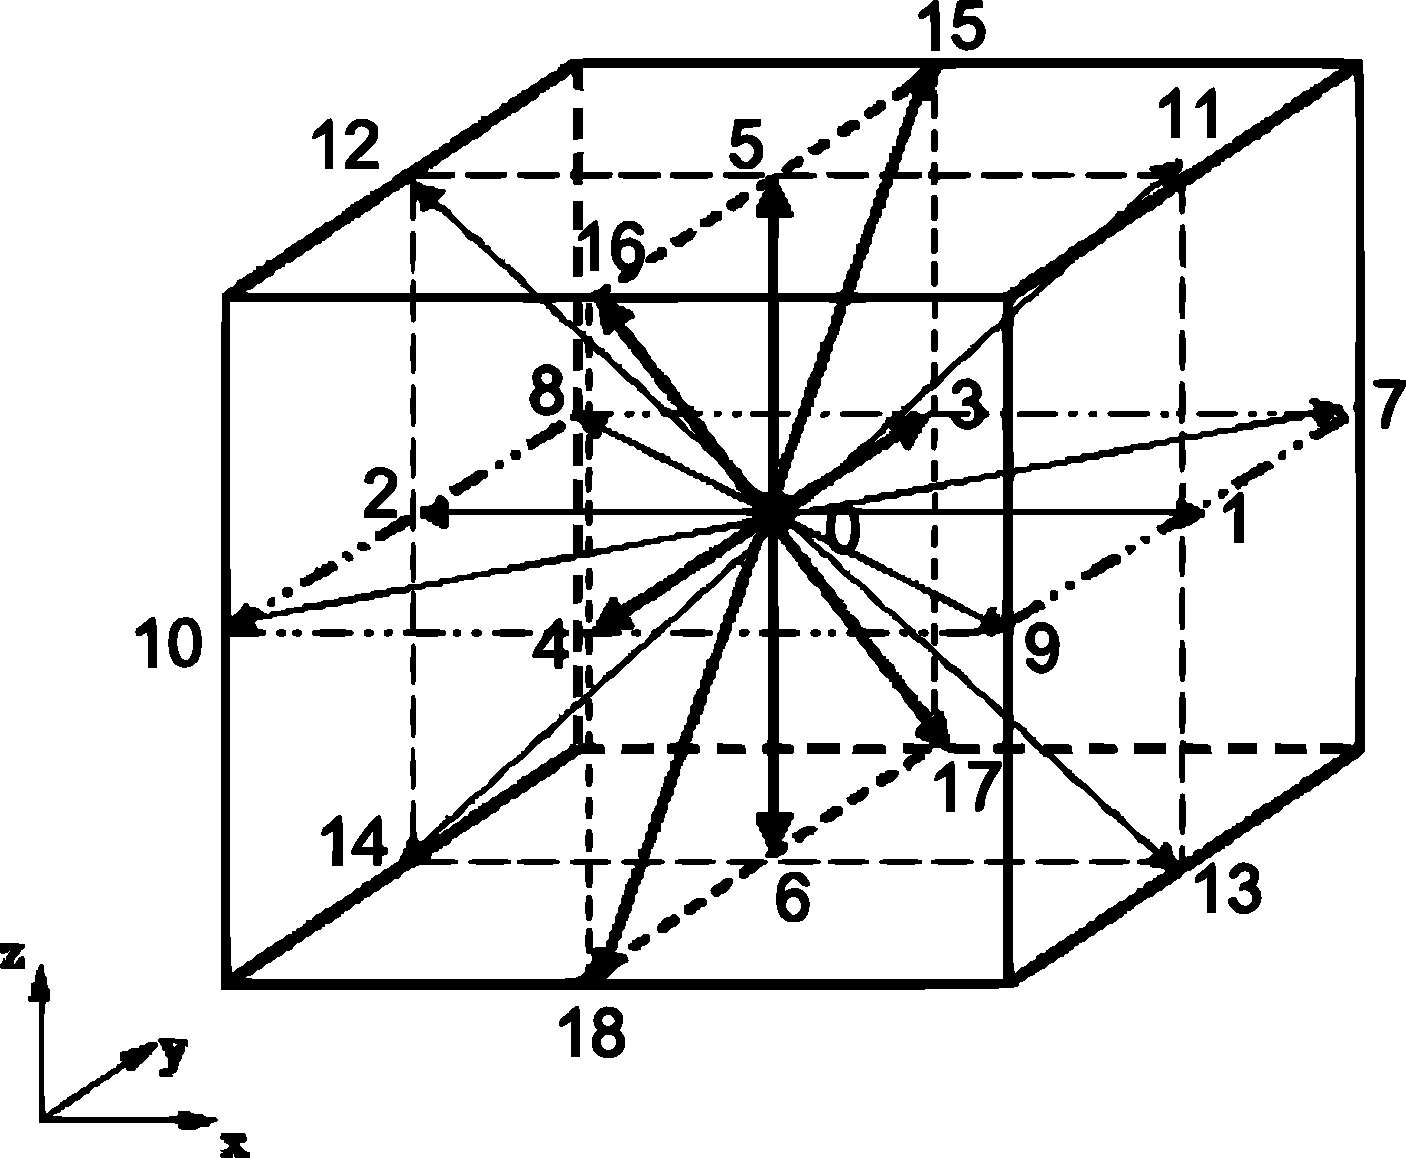
\includegraphics[width=.8\linewidth]{figuras/d3q19.pdf}
  \caption[Esquemático do D3Q19]{Esquemático do modelo D3Q19. Ilustração adaptada do estudo de \citeonline{premnath2013investigation}.}
  \label{fig:d3q19}
\end{figure}

Na Figura \ref{fig:d3q19} é possível visualizar espacialmente as direções de propagação da célula. Vale ressaltar que para cada direção há o cáculo da função de Maxwell ($f_{i}^{M}$) e, por conseguinte, a operação de propagação das funções de distribuição para a célula adjacente no sentido de cada direção.

\subsection{Múltiplos Tempos de Relaxação}

A equação \ref{eq:omega_i} retrata um operador de colisão com tempo de relaxação único. Essa abordagem é funcional porém, em regimes de pouca viscosidade cinemática como é o caso do ar, começa a desenvolver várias instabilidades e divergências como mostra o estudo de \citeonline{lallemand2000theory}. Para esses tipos de problemas a abordagem de múltiplos tempos de relaxação, \textit{multiple}-\textit{relaxation}-\textit{time} (MRT)\abreviatura{MRT}{\textit{multiple}-\textit{relaxation}-\textit{time}}, pode ser usada assim como é mostrado nos estudos de \citeonline{viggen2014lattice}.

De acordo com o esquema proposto por \citeonline{d1994generalized}, a formulação de MRT se baseia na troca do parâmetro de único tempo de relaxação $\tau$ por uma matriz \textbf{$\Lambda$} de vários tempos de relaxação. Todavia a matriz \textbf{$\Lambda$} é construída de acordo com uma matriz \textbf{$M$} que que projeta as funções de distribuição $f_{i}$ e $f_{i}^{M}$ no espaço dos momentos. De acordo com \citeonline{lallemand2000theory}, a possibilidade desse método ser mais estável é oriunda da capacidade de operar a colisão das células com um tempo de relaxação apropriado para cada um dos vários momentos, projetados a partir das funções de distribuição $f_{i}$ e $f_{i}^{M}$. Em vista do exposto o operador de colisão da equação \ref{eq:omega_i} se transforma em
\begin{equation}
	\Omega_{i} = -\textbf{$\Lambda$}(f_{i} - f_{i}^{M}).
    \label{eq:MRT_1}
\end{equation}
Porém a operação de colisão é realizada no espeço dos momentos, logo é preciso projetar $f_{i}$ e $f_{i}^{M}$ no espeço dos momentos ficando
\begin{equation}
	m_{i} = \textbf{$M$}f_{i} \text{ e } m_{i}^{M} = \textbf{$M$}f_{i}^{M}.
    \label{eq:MRT_2}
\end{equation}
Considerando que a matriz \textbf{$S$} é dada por
\begin{equation}
	\textbf{$S$} = \textbf{$M$}\textbf{$\Lambda$}\textbf{$M$}^{-1},
    \label{eq:MRT_3}
\end{equation}
o operador de colisão fica
\begin{equation}
	\Omega_{i} = -\textbf{$M$}^{-1}\textbf{$S$}(m_{i} - m_{i}^{M}).
    \label{eq:MRT_4}
\end{equation}
Inserindo a equação \ref{eq:MRT_4} na equação \ref{eq:f_i} fica
\begin{equation}
	f_{i}(\textbf{x} + c_{i}\Delta t, t + \Delta t) = f_{i}(\textbf{x}, t) -\textbf{$M$}^{-1}\textbf{$S$}(m_{i} - m_{i}^{M}).
    \label{eq:MRT_5}
\end{equation}
Vale ressaltar que a operação de propagação, lado esquerdo da equação \ref{eq:MRT_5}, ocorre no espaço original da função de distribuição $f_{i}$.

\subsection{Transformações para Unidades Físicas}

Quando as equações \ref{eq:rho}, \ref{eq:u}, \ref{eq:p} e \ref{eq:nu} são usadas para recuperar os atributos macroscópicos do fluido a unidade de medida não é uma unidade física. Segudo o trabalho de \citeonline{da2016prediction}, para se ter esses atributos em unidade física é preciso aplicar regras de conversão. Essas regras de conversão se baseiam em duas constantes que são definidas a partir de unidades físicas: velocidade característica definida por   
\begin{equation}
	\zeta = c^{*}/c_{s},
    \label{eq:conversao_1}
\end{equation}
tal que $c^{*}$ é a velocidade física do som, e discretização $\Delta x$ definida pela quantidade de metros por tamanho de célula.

Com os parâmetros $c^{*}$ e $\Delta x$ pode-se realizar as seguintes conversões para unidades físicas:
\begin{equation}
	\textbf{$u^{*}$} = \zeta \textbf{$u$}\text{, } \textbf{$x^{*}$} = \Delta x\textbf{$x$}
	\text{, } t^{*} = \frac{\Delta x}{\zeta}t \text{, } \nu^{*} = \zeta \textbf{x} \nu
	\text{, } \rho^{*} = \frac{\zeta}{\Delta x} \rho \text{ e } p^{*} = p \zeta^{2}  \rho_{0},
    \label{eq:conversao_1}
\end{equation}
tal que as variáveis assinaladas com $*$ são em unidades físicas e $\rho_{0}$ é unidade de densidade física ambiente.

\simbolo{$\rho_{0}$}{Unidade de densidade física ambiente}
